\documentclass[aps,pra,onecolumn,notitlepage,11pt,tightenlines,amsmath,amssymb,floatfix,longbibliography]{revtex4-2}

\usepackage[margin=0.70in]{geometry}
\usepackage{graphicx}
\usepackage{amsthm}
\usepackage{mathtools}
\usepackage{microtype}
\usepackage{hyperref}

% Flat-tarball and repository subdirectory figure resolution
\graphicspath{{figures/}{./}}

\hypersetup{
    colorlinks=true,
    linkcolor=blue,
    citecolor=blue,
    urlcolor=blue,
    pdftitle={Overcompleteness and Continuous Frame Properties of Physical Perfect Vortex Beams},
    pdfauthor={Sebasti\'an Ayala}
}

% Notation macros (all invoked in text)
\providecommand{\bra}[1]{\langle#1\rvert}
\providecommand{\ket}[1]{\lvert#1\rangle}
\providecommand{\braket}[2]{\langle#1\vert#2\rangle}
\providecommand{\abs}[1]{\lvert#1\rvert}
\providecommand{\norm}[1]{\lVert#1\rVert}

\newtheorem{theorem}{Theorem}
\newtheorem{proposition}{Proposition}
\newtheorem{corollary}{Corollary}
\newtheorem{remark}{Remark}

\begin{document}

\title{Overcompleteness and Continuous Frame Properties of Physical Perfect Vortex Beams}

\author{Sebasti\'an Ayala}
\email{ayala.phys.ds@gmail.com}
\thanks{ORCID: \href{https://orcid.org/0009-0003-7348-3883}{0009-0003-7348-3883}}
\affiliation{Independent Researcher, Cauquenes, Chile}

\date{\today}

\begin{abstract}
Physical perfect optical vortex beams (PVBs) possess an annular intensity profile of finite thickness $w > 0$ whose ring radius $R$ is nominally independent of the orbital angular momentum topological charge $l$. Here, we establish their operator-theoretic structure as continuous Hilbert frames. While azimuthal modes remain strictly orthogonal ($\delta_{l,l'}$), radial nonorthogonality induces a frame operator $S_w$ acting as an isotropic Gaussian convolution $G_w * \cdot$, yielding a vanishing global lower bound ($A = 0$) on $L^2(\mathbb{R}^2)$. Restricted to the paraxial Paley--Wiener subspace $\mathcal{H}_{k_{\max}}$, PVBs form a stable frame with sharp bounds $A = \exp(-w^2 k_{\max}^2/2)$ and $B = 1$. We construct the projected Tikhonov-regularized canonical dual frame $S_{w,\alpha_{\mathrm{reg}}}^{-1}$, derive an exact $(p+1)$-term closed-form expansion $c_{l,p}(R)$ for arbitrary Laguerre--Gaussian ($\mathrm{LG}_{p,l}$) modes ($p \ge 0$), and establish the revised radial Rayleigh limit $w_{\mathrm{crit}} \approx 0.573\,w_0/\sqrt{2p+\abs{l}+1}$ ($p \ge 1$). For discrete radial multiplexing, normalized Gram conditioning converges monotonically ($\kappa(\gamma) = 1.645$ at $\Delta R = 2.0w$, $17.36\,\mathrm{dB}$ power isolation). Finally, we demonstrate quantitative classical and quantum utility: $259\times$ noisy $\mathrm{LG}_{2,1}$ mean-square-error suppression, $6.90\,\mathrm{dB}$ ring-core fiber coupling gain with $\le 0.42\,\mathrm{dB}$ ($N=6$) equalization penalty, Kolmogorov turbulence filtering, passive Gouy-diverse IC-POVM radial qudit tomography (rank $16/16$), and circular-iris Bell--CHSH preservation ($S_{\mathrm{PVB}} = 2.828$).
\end{abstract}

\maketitle

\section{Introduction}
\label{sec:intro}

Optical fields carrying orbital angular momentum (OAM) have transformed classical and quantum photonics since Allen \emph{et al.} showed that paraxial modes with azimuthal phase $\exp(il\phi)$ carry $l\hbar$ of OAM per photon~\cite{Allen1992}. The unbounded integer charge $l \in \mathbb{Z}$ underpins terabit space-division multiplexing (SDM)~\cite{Bozinovic2013,Willner2015,Wang2019}, optical trapping~\cite{Padgett2011}, and high-dimensional quantum cryptography and entanglement certification~\cite{Cerf2002,Mirhosseini2015,Bavaresco2018,Erhard2018}.

In conventional Laguerre--Gaussian ($\mathrm{LG}_{p,l}$) eigenmodes of waist $w_0$, the second-moment root-mean-square (RMS) beam radius scales as $r_{\mathrm{rms}} = w_0\sqrt{2p+\abs{l}+1}$~\cite{Allen1992,Siegman1986} (while for $p=0,\abs{l}\ge 1$ the peak ring radius lies at $r_{\mathrm{peak}} = w_0\sqrt{\abs{l}/2}$). This $l$-dependent expansion causes severe clipping and asymmetric insertion loss when launching OAM channels into fixed-annulus ring-core fibers (RCFs)~\cite{Ramachandran2009,Brunet2014,Gregg2015,Canas2021,RojasRojas2021,Villalba2023}. To decouple ring size from topological charge, Ostrovsky \emph{et al.} introduced the perfect optical vortex beam (PVB)~\cite{Ostrovsky2013,Vaity2015}, whose ideal Dirac limit $\Phi_{l,R}^{\mathrm{ideal}}(r,\phi) = (2\pi)^{-1/2} R^{-1}\delta(r-R)e^{il\phi}$ forms a generalized orthonormal basis in a rigged Hilbert space~\cite{Gelfand1964}. Realistic laboratory PVBs, however, necessarily carry finite radial half-width $w > 0$ and finite power~\cite{Vaity2015,Reddy2016}.

Recently, Ferreira \emph{et al.}~\cite{Ferreira2026} (Appendix~D) noted that finite-width PVBs fail orthogonality and induce Gaussian smoothing, computing the radial projection solely for $p=0$ while leaving $p \ge 1$ open. Four fundamental questions remained unresolved: (i) the operator-theoretic classification of physical PVBs in continuous frame theory~\cite{Duffin1952,Daubechies1990,Ali1993,Christensen2016} alongside Glauber coherent states~\cite{Klauder1985,Perelomov1986,Gazeau2009}; (ii) sharp stability bounds and regularized dual-frame inversion under noise; (iii) an exact closed-form expansion $c_{l,p}(R)$ for all $\mathrm{LG}_{p,l}$ modes ($p \ge 0$) and its nodal washout limit; and (iv) discrete Gram bounds and quantitative classical/quantum optics protocols.

Here, we resolve all four questions. Section~\ref{sec:pvb_formation} covers PVB scaling (Sec.~\ref{subsec:pvb_def}), $2f$ generation, and telecom/self-healing parameters (Sec.~\ref{subsec:pvb_generation}). Section~\ref{sec:frame_formalism} establishes azimuthal--radial decoupling (Sec.~\ref{subsec:overlap_kernel}), the Gaussian convolution kernel (Sec.~\ref{subsec:frame_operator}), and Paley--Wiener bounds (Sec.~\ref{subsec:paley_wiener}). Section~\ref{sec:properties} develops the Tikhonov dual (Sec.~\ref{subsec:tikhonov_dual}), the exact $\mathrm{LG}_{p,l}$ expansion (Sec.~\ref{subsec:analytic_lg_expansion} and Appendix~\ref{app:lg_expansion}), the radial Rayleigh limit (Sec.~\ref{subsec:nodal_washout}), and normalized Gram conditioning (Sec.~\ref{subsec:gram_sampling}). Section~\ref{sec:optics_utility} demonstrates classical (Sec.~\ref{subsec:classical_utility}) and quantum (Sec.~\ref{subsec:quantum_utility}) utility, and Sec.~\ref{sec:conclusions} concludes.

\section{Physical PVBs: Definition and Generation}
\label{sec:pvb_formation}

\subsection{Complex Field and Resolution-of-Identity Scaling}
\label{subsec:pvb_def}

In cylindrical coordinates $\mathbf{r} = (r,\phi)$ at the waist plane $z=0$, a physical PVB of topological charge $l \in \mathbb{Z}$, ring radius $R > 0$, and annular half-width $w > 0$ is~\cite{Ostrovsky2013,Vaity2015}
\begin{equation}
\Phi_{l,R}(r,\phi) = C_0 e^{il\phi} \exp\!\left(-\frac{r^2 + R^2}{w^2}\right) I_{\abs{l}}\!\left(\frac{2Rr}{w^2}\right),
\label{eq:pvb_mode}
\end{equation}
where $I_{\abs{l}}$ is the modified Bessel function of the first kind ($I_l(x) = I_{\abs{l}}(x)$ for $l \in \mathbb{Z}$) and
\begin{equation}
C_0 = \frac{1}{w^2}\sqrt{\frac{2}{\pi}}.
\label{eq:C0_norm}
\end{equation}
Crucially, $C_0$ carries dimensions $[\mathrm{length}^{-2}]$ and is \emph{not} an $L^2(\mathbb{R}^2)$ normalization constant; rather, it is the continuous-frame resolution-of-identity scaling fixing the upper frame bound $B = 1$ under radial measure $d\mu(R) = R\,dR$. Its squared norm is $\norm{\Phi_{l,R}}_{L^2}^2 = w^{-2} e^{-R^2/w^2} I_{\abs{l}}(R^2/w^2) < w^{-2}$ (e.g., $\norm{\Phi_{1,2}}_{L^2}^2 = 0.3894 \neq 1$ at $R=2.0\,\ell_0, w=0.5\,\ell_0$). Unit-normalized channel states are $\psi_{l,R} = \Phi_{l,R}/\norm{\Phi_{l,R}}_{L^2}$. We restrict the annular regime to $R > 0$: at $R=0$, $\Phi_{l,0} \equiv 0$ for all $l \neq 0$, whereas $l=0$ degenerates to the on-axis Gaussian $\Phi_{0,0}(r) = C_0 e^{-r^2/w^2}$ with $\norm{\Phi_{0,0}}_{L^2}^2 = 1/w^2$ (of zero $R\,dR$ measure).

Using Hankel's expansion $I_{\abs{l}}(x) = \frac{e^x}{\sqrt{2\pi x}}[1 - \frac{4l^2-1}{8x} + \mathcal{O}(x^{-2})]$ with $x = 2Rr/w^2$, Eq.~\eqref{eq:pvb_mode} reduces to~\cite{Ferreira2026}
\begin{equation}
\Phi_{l,R}(r,\phi) \approx \frac{e^{il\phi}}{\sqrt{2\pi^2 R r\, w^2}} \exp\!\left[-\frac{(r - R)^2}{w^2}\right],
\label{eq:pvb_asymptotic}
\end{equation}
valid uniformly in the annular region $r \sim R \gg w$ and $\abs{l} \ll 2R/w$ (equivalently $l^2 \ll 4Rr/w^2$). Away from the ring ($r \to 0$), Eq.~\eqref{eq:pvb_asymptotic} diverges as $r^{-1/2}$ whereas Eq.~\eqref{eq:pvb_mode} vanishes as $r^{\abs{l}}$; even at $R/w = 4, l = 4$ ($x=32$), the leading-order relative error reaches $28.4\%$. Maximizing $\abs{\Phi_{l,R}(r)}^2$ yields the transcendental peak condition $r_{\mathrm{peak}} = R[\abs{l}/x + I_{\abs{l}+1}(x)/I_{\abs{l}}(x)]$, giving a small topological shift $\Delta r_{\mathrm{peak}}/R \approx (l^2/8)(w/R)^4$ for $w \ll R$ [Fig.~\ref{fig:frame_spectrum}(a)].

\subsection{Optical Generation, Telecom Bridge, and Propagation}
\label{subsec:pvb_generation}

A physical PVB is generated as the $2f$ optical Fourier transform of a Bessel--Gaussian (BG) beam~\cite{Gori1987,Vaity2015}:
\begin{equation}
E_{\mathrm{BG}}(\rho,\theta) = E_0 J_l(k_r\rho)\exp\!\left(-\frac{\rho^2}{w_g^2}\right) e^{il\theta},
\label{eq:bg_field}
\end{equation}
where $k_r = k_0(n_{\mathrm{ax}}-1)\beta$, $k_0 = 2\pi/\lambda$ is the optical wavenumber, $w_g$ is the Gaussian waist, and $\beta$ is the axicon base (wedge) angle (full opening angle $\pi - 2\beta$). Placing the BG waist at input distance $d_{\mathrm{in}} = f$ before a lens of focal length $f$ cancels the residual quadratic chirp $\exp[i k_0 r^2(1-d_{\mathrm{in}}/f)/(2f)]$, yielding at the back focal plane ($z=2f$)~\cite{Vaity2015,Villalba2023}
\begin{equation}
R = \frac{k_r f}{k_0} = (n_{\mathrm{ax}}-1)\beta f, \qquad w = \frac{2f}{k_0 w_g},
\label{eq:fourier_parameters}
\end{equation}
with overall Fourier phase $(-i)^{l+1} e^{2ik_0 f}$ from signed $J_l(k_r\rho)$ in Eq.~\eqref{eq:bg_field} [or $(-i)^{\abs{l}+1} e^{2ik_0 f}$ if $J_{\abs{l}}(k_r\rho)$ is used]. Because the BG focal amplitude scales as $E_0 w_g / w \propto w^{-1}$ at fixed $E_0$, matching $C_0$ in Eq.~\eqref{eq:C0_norm} requires rescaling $E_0 = \sqrt{2/\pi}/(w w_g) = k_0/(\sqrt{2\pi}\,f)$ (input power $P_{\mathrm{in}} = \norm{\Phi_{l,R}}_{L^2}^2 \propto w^{-1}$ for $R \gg w$).

Using phase-only spatial light modulators (SLMs), Rojas-Rojas \emph{et al.} predicted $>99.5\%$ theoretical coupling efficiency into RCFs~\cite{RojasRojas2021}, while Villalba \emph{et al.} demonstrated experimentally across $l=1\text{--}6$ a $15\times$ reduction in ring-radius variance, a $6.83\,\mathrm{dB}$ coupling gain over $\mathrm{LG}$ modes at $l=4$, and $1\,\mathrm{Gbps}$ transmission over $300\,\mathrm{m}$ of RCF~\cite{Villalba2023}. Substituting telecom parameters ($\lambda = 1550\,\mathrm{nm}$, $k_0 = 4.054\times 10^6\,\mathrm{m}^{-1}$, collection numerical aperture $\mathrm{NA} = 0.20 \implies k_{\max} = k_0 \mathrm{NA} = 8.107\times 10^5\,\mathrm{m}^{-1}$, and RCF-matched $w = 1.72\,\mu\mathrm{m}$) into Eq.~\eqref{eq:fourier_parameters} yields the dimensionless bandwidth product $w k_{\max} = 1.394$, anchoring our frame bounds in Fig.~\ref{fig:frame_spectrum}(d).

\begin{remark}[Fresnel propagation (\texorpdfstring{$z>0$}{z > 0}) and self-healing]
\label{rem:propagation}
Under paraxial Fresnel propagation past the focal waist ($z>0$), the annular thickness $w$ remains quasi-invariant over the ring Rayleigh depth $z_R^{\mathrm{ring}} \sim k_0 w^2/2$, while the conical BG wavevectors ($\sin\gamma = k_r/k_0$) enable geometric self-healing past an on-axis obstacle of radius $a_{\mathrm{obs}} \lesssim R$ at distance $z_{\mathrm{heal}} \approx R/\sin\gamma = k_0 R/k_r$, within the axicon zone $z_{\max} \approx k_0 w_g/k_r$.
\end{remark}

\section{Continuous Hilbert Frame Formalism}
\label{sec:frame_formalism}

\subsection{Azimuthal--Radial Decoupling and Mutual Overlap}
\label{subsec:overlap_kernel}

Because azimuthal OAM eigenphases $e^{il\phi}/\sqrt{2\pi}$ are mutually orthonormal, the transverse Hilbert space decomposes into an orthogonal direct sum of azimuthal sectors:
\begin{align}
\mathcal{H} &= L^2(\mathbb{R}^2) = \bigoplus_{l\in\mathbb{Z}} \mathcal{H}_l, \nonumber \\
\mathcal{H}_l &= \left\{ f(r)\frac{e^{il\phi}}{\sqrt{2\pi}} : \int_0^\infty \abs{f(r)}^2 r\,dr < \infty \right\}.
\label{eq:direct_sum}
\end{align}
Any overcompleteness of physical PVBs resides strictly in the radial coordinate $R > 0$ within each $\mathcal{H}_l$ of Eq.~\eqref{eq:direct_sum}. Computing the $L^2(\mathbb{R}^2)$ inner product between $\Phi_{l,R}$ and $\Phi_{l',R'}$ gives
\begin{align}
\braket{\Phi_{l,R}}{\Phi_{l',R'}} &= C_0^2 \int_0^{2\pi} d\phi\, e^{i(l'-l)\phi} \int_0^\infty r\,dr\, e^{-\frac{2r^2+R^2+R'^2}{w^2}} \nonumber \\
&\quad \times I_{\lvert l\rvert}\!\left(\frac{2Rr}{w^2}\right) I_{\lvert l'\rvert}\!\left(\frac{2R'r}{w^2}\right),
\label{eq:overlap_start}
\end{align}
where the azimuthal integral yields $2\pi\delta_{l,l'}$ [Fig.~\ref{fig:frame_spectrum}(b) inset]. Setting $l'=l$ in Eq.~\eqref{eq:overlap_start} and invoking $I_l = I_{\abs{l}}$ ($\operatorname{Re}(\abs{l}) \ge 0 > -1$) permits applying Weber's exponential integral, formula 6.633.2 of Gradshteyn and Ryzhik~\cite{Gradshteyn2014} (analytically continued via $J_\nu(ix)=i^\nu I_\nu(x)$, valid for $\operatorname{Re}(p)>0, \operatorname{Re}(\nu)>-1$),
\begin{equation}
\int_0^\infty x\, e^{-px^2} I_\nu(ax) I_\nu(bx)\,dx = \frac{1}{2p} e^{\frac{a^2+b^2}{4p}} I_\nu\!\left(\frac{ab}{2p}\right),
\label{eq:weber_identity}
\end{equation}
with $p = 2/w^2$, $a = 2R/w^2$, and $b = 2R'/w^2$. Substituting Eq.~\eqref{eq:C0_norm} yields
\begin{equation}
\braket{\Phi_{l,R}}{\Phi_{l',R'}} = \delta_{l,l'}\,\frac{1}{w^2}\exp\!\left(-\frac{R^2 + R'^2}{2w^2}\right) I_{\abs{l}}\!\left(\frac{RR'}{w^2}\right),
\label{eq:overlap_closed}
\end{equation}
confirming strict Kronecker orthogonality across $l$ and strictly positive radial overlap $\gamma_l(R,R') = \braket{\Phi_{l,R}}{\Phi_{l,R'}}/\allowbreak(\norm{\Phi_{l,R}}\norm{\Phi_{l,R'}})$ [Fig.~\ref{fig:frame_spectrum}(b)].

\begin{figure}[htbp]
\centering
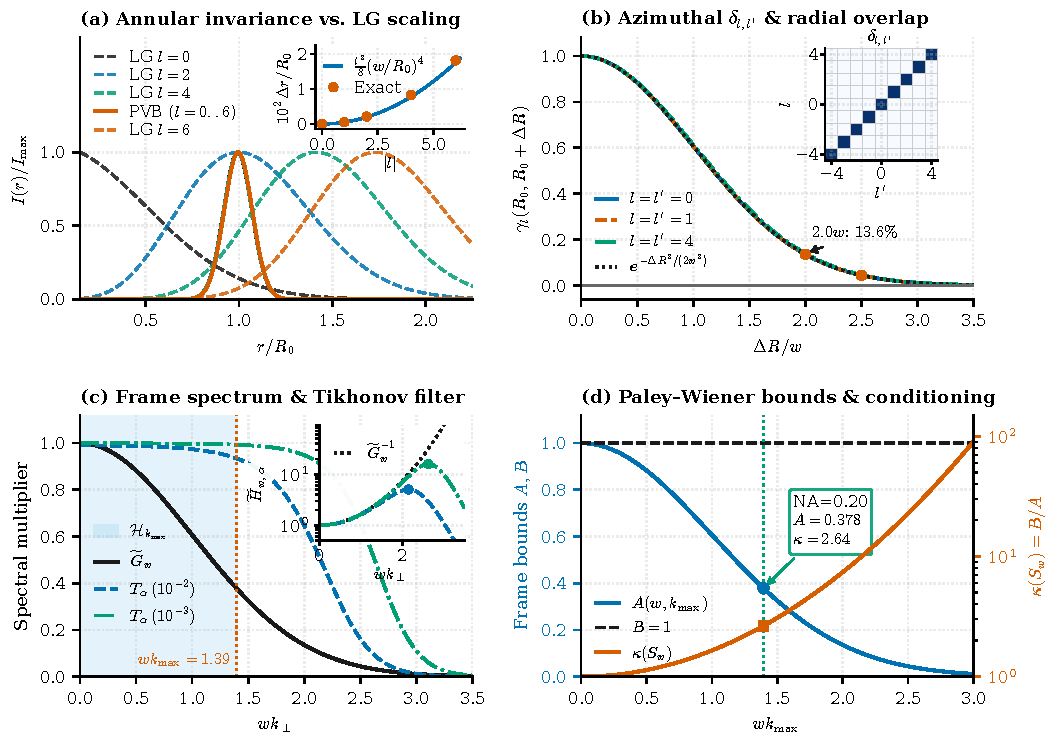
\includegraphics[width=0.76\textwidth]{fig1_frame_spectrum.pdf}
\caption{Physical PVB continuous frame structure and spectrum. (a) Normalized radial intensity $I(r)/I_{\max}$ for PVBs ($w/R_0 = 0.15$, solid) across $l = 0,2,4,6$ vs.\ $\mathrm{LG}_{0,l}$ ($w_0 = R_0$, dashed); inset compares the transcendental peak shift $\Delta r/R_0$ ($w/R_0 = 0.25$, circles) with $(l^2/8)(w/R_0)^4$. (b) Normalized radial overlap $\gamma_l(R_0, R_0+\Delta R)$ at $R_0 = 4w$ for $l=0,1,4$ vs.\ $e^{-\Delta R^2/(2w^2)}$ (dotted), marking $13.6\%$ at $2.0w$ and $4.40\%$ at $2.5w$; inset shows azimuthal orthogonality $\delta_{l,l'}$. (c) Spectral multiplier $\widetilde{G}_w(k_\perp)$ and Tikhonov transfer $T_{\alpha_{\mathrm{reg}}}(k_\perp)$ ($\alpha_{\mathrm{reg}} = 10^{-2}, 10^{-3}$) with $\mathcal{H}_{k_{\max}}$ shaded up to $w k_{\max} = 1.39$; inset shows noise gain $\widetilde{H}_{w,\alpha_{\mathrm{reg}}}$ peaking at $(2\sqrt{\alpha_{\mathrm{reg}}})^{-1}$. (d) Paley--Wiener bounds $A(w,k_{\max}), B=1$ and $\kappa(S_w)$ vs.\ $w k_{\max}$, marking the telecom benchmark ($\lambda=1550\,\mathrm{nm}, \mathrm{NA}=0.20, w=1.72\,\mu\mathrm{m}$: $A=0.378, \kappa=2.64$).}
\label{fig:frame_spectrum}
\end{figure}

\subsection{Continuous Frame Operator and Convolution Kernel}
\label{subsec:frame_operator}

A family $\{\Phi_\omega\}_{\omega\in\Omega}$ in $\mathcal{H}$ with measure $\mu$ forms a continuous Hilbert frame~\cite{Duffin1952,Daubechies1990,Ali1993,Christensen2016} if there exist $0 < A \le B < \infty$ such that for all $\psi \in \mathcal{H}$,
\begin{equation}
A \norm{\psi}_{L^2}^2 \le \int_\Omega \abs{\braket{\Phi_\omega}{\psi}}^2\,d\mu(\omega) \le B \norm{\psi}_{L^2}^2.
\label{eq:frame_def}
\end{equation}
With $\Omega = \mathbb{Z} \times (0,\infty)$ and $d\mu(l,R) = R\,dR$, the PVB frame operator $S_w: \mathcal{H} \to \mathcal{H}$ is
\begin{equation}
S_w\psi = \sum_{l\in\mathbb{Z}} \int_0^\infty R\,dR\, \braket{\Phi_{l,R}}{\psi}\Phi_{l,R}.
\label{eq:frame_op}
\end{equation}
We adopt the non-unitary 2D Fourier transform convention
\begin{align}
\widetilde{\psi}(\mathbf{k}) &= \int_{\mathbb{R}^2} \psi(\mathbf{r}) e^{-i\mathbf{k}\cdot\mathbf{r}}\,d^2\mathbf{r}, \nonumber \\
\psi(\mathbf{r}) &= \int_{\mathbb{R}^2} \widetilde{\psi}(\mathbf{k}) e^{i\mathbf{k}\cdot\mathbf{r}}\,\frac{d^2\mathbf{k}}{(2\pi)^2},
\label{eq:ft_convention}
\end{align}
with transverse spatial frequency $k_\perp = \abs{\mathbf{k}} = \sqrt{k_x^2 + k_y^2}$.

\begin{proposition}[Azimuthal--radial decoupling and Gaussian kernel]
\label{prop:conv_kernel}
For any $w > 0$, the PVB family $\{\Phi_{l,R}\}_{l\in\mathbb{Z},\,R>0}$ obeys Eq.~\eqref{eq:overlap_closed}, and its frame operator~\eqref{eq:frame_op} acts on $L^2(\mathbb{R}^2)$ as the isotropic Gaussian convolution $(S_w\psi)(\mathbf{r}) = (G_w * \psi)(\mathbf{r})$ with $G_w(\mathbf{r}) = (2\pi w^2)^{-1}\exp(-\abs{\mathbf{r}}^2/(2w^2))$, diagonalized in Fourier space as $\widetilde{(S_w\psi)}(\mathbf{k}) = \exp(-w^2 k_\perp^2/2)\widetilde{\psi}(\mathbf{k})$.
\end{proposition}
\begin{proof}
Using the Jacobi--Anger expansion and Eq.~\eqref{eq:weber_identity} analytically continued to $J_{\abs{l}}$, the 2D Fourier transform~\eqref{eq:ft_convention} of Eq.~\eqref{eq:pvb_mode} is
\begin{equation}
\widetilde{\Phi}_{l,R}(\mathbf{k}) = \sqrt{2\pi}\,(-i)^{\abs{l}} e^{il\phi_k} \exp\!\left(-\frac{w^2 k_\perp^2}{4}\right) J_{\abs{l}}(R k_\perp).
\label{eq:pvb_ft}
\end{equation}
Applying Plancherel's identity $\braket{\Phi_{l,R}}{\psi} = (2\pi)^{-2}\braket{\widetilde{\Phi}_{l,R}}{\widetilde{\psi}}$ to the Fourier transform of Eq.~\eqref{eq:frame_op}, the radial integral collapses via Hankel closure $\int_0^\infty R\,dR\,J_{\abs{l}}(Rk_\perp)J_{\abs{l}}(Rk_\perp') = \delta(k_\perp - k_\perp')/k_\perp$, and the azimuthal sum collapses via $\frac{1}{2\pi}\sum_{l\in\mathbb{Z}} e^{il(\phi_k-\phi_{k'})} = \delta(\phi_k - \phi_{k'})$, yielding
\begin{equation}
\widetilde{(S_w\psi)}(\mathbf{k}) = \widetilde{G}_w(k_\perp)\widetilde{\psi}(\mathbf{k}), \quad \widetilde{G}_w(k_\perp) = \exp\!\left(-\frac{w^2 k_\perp^2}{2}\right).
\label{eq:fourier_diag}
\end{equation}
Inverse Fourier transformation gives $(S_w\psi)(\mathbf{r}) = (G_w * \psi)(\mathbf{r})$ with $G_w(\mathbf{r}) = (2\pi w^2)^{-1}e^{-\abs{\mathbf{r}}^2/(2w^2)}$, recovering the convolution action noted in Appendix~D of Ref.~\cite{Ferreira2026}.
\end{proof}

\subsection{Paley--Wiener Bounds and Physical Obstructions to \texorpdfstring{$w \to 0$}{w -> 0}}
\label{subsec:paley_wiener}

Restricting to the paraxial Paley--Wiener subspace of optical fields bandlimited by $k_{\max} = k_0 \mathrm{NA}$,
\begin{align}
\mathcal{H}_{k_{\max}} &= \left\{\psi \in L^2(\mathbb{R}^2) : \operatorname{supp}(\widetilde{\psi}) \subseteq \{\abs{\mathbf{k}} \le k_{\max}\}\right\} \nonumber \\
&= \bigoplus_{l\in\mathbb{Z}} \mathcal{H}_{l,k_{\max}},
\label{eq:paley_wiener}
\end{align}
and letting $P_{k_{\max}}\psi = \mathcal{F}^{-1}\{\mathbf{1}_{k_\perp \le k_{\max}}\widetilde{\psi}\}$ denote its orthogonal projector, Proposition~\ref{prop:conv_kernel} yields the following frame stability theorem.

\begin{theorem}[Paley--Wiener frame stability and projected canonical dual]
\label{thm:pw_bounds}
(i) On unconstrained $L^2(\mathbb{R}^2)$, $\{\Phi_{l,R}\}$ is a continuous Bessel system with optimal upper bound $B=1$ and vanishing lower bound $A = \inf_{k_\perp \ge 0} \widetilde{G}_w(k_\perp) = 0$; consequently, $S_w^{-1}$ is unbounded and $S_w^{-1}\Phi_{l,R} \notin L^2(\mathbb{R}^2)$. (ii) On $\mathcal{H}_{k_{\max}}$ of Eq.~\eqref{eq:paley_wiener}, the projected family $\{P_{k_{\max}}\Phi_{l,R}\}$ forms a continuous Hilbert frame satisfying Eq.~\eqref{eq:frame_def} with frame operator $S_{w,k_{\max}} = P_{k_{\max}} S_w P_{k_{\max}}$, sharp bounds
\begin{equation}
A(w, k_{\max}) = \exp\!\left(-\frac{w^2 k_{\max}^2}{2}\right), \qquad B = 1,
\label{eq:optimal_bounds}
\end{equation}
spectral condition number $\kappa(S_{w,k_{\max}}) = B/A = \exp(w^2 k_{\max}^2/2)$, and well-defined canonical dual modes $\widetilde{\Phi}_{l,R} = S_{w,k_{\max}}^{-1} P_{k_{\max}}\Phi_{l,R} \in \mathcal{H}_{k_{\max}}$.
\end{theorem}
\begin{proof}
By Plancherel's theorem and Eq.~\eqref{eq:fourier_diag}, $\braket{\psi}{S_w\psi} = (2\pi)^{-2}\int_{\mathbb{R}^2} e^{-w^2 k_\perp^2/2}\abs{\widetilde{\psi}(\mathbf{k})}^2\,d^2\mathbf{k}$. On $\mathcal{H}_{k_{\max}}$,
\begin{equation}
e^{-w^2 k_{\max}^2/2} \le \widetilde{G}_w(k_\perp) \le 1 \qquad (\forall\, k_\perp \in [0, k_{\max}]),
\label{eq:transfer_bounds}
\end{equation}
establishing Eq.~\eqref{eq:optimal_bounds} directly from Eq.~\eqref{eq:transfer_bounds}. To prove sharpness on $\mathcal{H}_{k_{\max}}$, consider the normalized Fourier-ring test families $\widetilde{\psi}_\epsilon^{(+)}(\mathbf{k}) \propto \mathbf{1}_{\{0 < k_\perp \le \epsilon\}}$ and $\widetilde{\psi}_\epsilon^{(-)}(\mathbf{k}) \propto \mathbf{1}_{\{k_{\max}-\epsilon \le k_\perp \le k_{\max}\}}$ ($\epsilon \in (0, k_{\max})$); taking $\epsilon \to 0^+$ yields $\braket{\psi_\epsilon^{(+)}}{S_w\psi_\epsilon^{(+)}} \to 1 = B$ and $\braket{\psi_\epsilon^{(-)}}{S_w\psi_\epsilon^{(-)}} \to A(w,k_{\max})$ (and $k_{\max} \to \infty$ gives $A=0$ on $L^2$). Because $\widetilde{\Phi}_{l,R}(\mathbf{k})$ in Eq.~\eqref{eq:pvb_ft} has unbounded support, $\Phi_{l,R} \notin \mathcal{H}_{k_{\max}}$ and $e^{+w^2 k_\perp^2/2}\widetilde{\Phi}_{l,R}(\mathbf{k}) \notin L^2(\mathbb{R}^2)$, so only the projected dual $S_{w,k_{\max}}^{-1}P_{k_{\max}}\Phi_{l,R} \in \mathcal{H}_{k_{\max}}$ exists.
\end{proof}

Notice that $\mathcal{H}_{k_{\max}}$ is a reproducing-kernel Hilbert space (RKHS)~\cite{PaulsenRaghupathi2016} with bandlimited Bessel kernel, and that physical realizability forbids taking the ideal Dirac limit $w \to 0$: (i) transverse wavevector variance scales as $\langle k_\perp^2 \rangle \sim w^{-2} \to \infty$, violating paraxiality; (ii) beam quality degrades as $M^2 \sim R/w \to \infty$; (iii) finite aperture diameter $D$ enforces the diffraction cutoff $w \ge 2\lambda f/(\pi D)$; and (iv) $\Phi_{l,R}^{\mathrm{ideal}} \notin L^2(\mathbb{R}^2)$ exists solely in the dual $\Phi^\times$ of a Gel'fand rigged Hilbert triplet $\Phi \subset L^2(\mathbb{R}^2) \subset \Phi^\times$~\cite{Gelfand1964}. Table~\ref{tab:frame_comparison} contrasts physical PVBs with Dirac PVBs, $\mathrm{LG}_{p,l}$ modes, and Glauber coherent states $\ket{\alpha}$~\cite{Klauder1985,Perelomov1986,Gazeau2009}.

\begin{table}[htbp]
\caption{Comparison of optical mode families and continuous frames across function space, orthogonality, completeness bounds, dual inversion, and waveguide/pupil footprint.}
\label{tab:frame_comparison}
\begin{ruledtabular}
\footnotesize
\begin{tabular}{p{2.3cm}p{3.2cm}p{4.3cm}p{3.4cm}p{3.4cm}}
Property & Ideal Dirac PVB ($w=0$) & Physical PVB ($w>0$) & $\mathrm{LG}_{p,l}$ Modes & Coherent States $\ket{\alpha}$ \\
\hline
Function space & Rigged dual $\Phi^\times$ ($\notin L^2$) & $L^2(\mathbb{R}^2)$ (frame on $\mathcal{H}_{k_{\max}}$) & $L^2(\mathbb{R}^2)$ (complete ONB) & Bargmann--Fock $L^2$ \\
Orthogonality & $\delta_{l,l'}\delta(R-R')/R$ & $\delta_{l,l'}$ in $l$; $\gamma_l(R,R')>0$ in $R$ & $\delta_{p,p'}\delta_{l,l'}$ (orthogonal) & $\abs{\braket{\alpha}{\beta}} = e^{-\abs{\alpha-\beta}^2/2}$ \\
Completeness / bounds & Generalized ONB & $A = e^{-w^2 k_{\max}^2/2},\, B=1$ ($\mathcal{H}_{k_{\max}}$) & Tight ($A=B=1$) & Tight ($A=B=1$, measure $d^2\alpha/\pi$) \\
Dual / inversion & Self-dual ($\notin L^2$) & $S_w = G_w * \cdot$; projected / Tikhonov dual & Self-dual ($S=\mathbb{I}$) & Self-dual ($S=\mathbb{I}$) \\
Pupil / RCF footprint & Singular (infinite $k_\perp$ variance) & $l$-invariant ring $R$ ($\bar{\eta}_l = 98.5\%$ in RCF) & $r_{\mathrm{rms}} = w_0\sqrt{2p+\abs{l}+1}$ ($l$-clipping) & Displaced phase-space packet \\
\end{tabular}
\end{ruledtabular}
\end{table}

\section{Core Properties of the Overcomplete PVB Frame}
\label{sec:properties}

\subsection{Projected and Tikhonov-Regularized Canonical Dual Frames}
\label{subsec:tikhonov_dual}

Under noisy optical detection, $\psi_{\mathrm{meas}}(\mathbf{r}) = (S_w\psi)(\mathbf{r}) + \eta(\mathbf{r})$, applying the unregularized inverse $\widetilde{G}_w^{-1}(k_\perp) = \exp(+w^2 k_\perp^2/2)$ amplifies high-frequency noise $\widetilde{\eta}(\mathbf{k})$ exponentially. To stabilize reconstruction over $\mathcal{H} \in \{L^2(\mathbb{R}^2), \mathcal{H}_{k_{\max}}\}$, we solve the Tikhonov variational problem with dimensionless regularization parameter $\alpha_{\mathrm{reg}} > 0$:
\begin{equation}
\min_{\psi \in \mathcal{H}} \left\{ \norm{S_w\psi - \psi_{\mathrm{meas}}}_{L^2}^2 + \alpha_{\mathrm{reg}}\norm{\psi}_{L^2}^2 \right\}.
\label{eq:tikhonov_opt}
\end{equation}

\begin{proposition}[Tikhonov-regularized dual frame and noise-gain peak]
\label{prop:tikhonov_dual}
For any $\alpha_{\mathrm{reg}} > 0$, the unique minimizer of Eq.~\eqref{eq:tikhonov_opt} defines the bounded inverse $S_{w,\alpha_{\mathrm{reg}}}^{-1} = (S_w^2 + \alpha_{\mathrm{reg}}\mathbb{I})^{-1}S_w$, regularized dual modes $\widetilde{\Phi}_{l,R}^{(\alpha_{\mathrm{reg}})} = S_{w,\alpha_{\mathrm{reg}}}^{-1}\Phi_{l,R} \in L^2(\mathbb{R}^2)$ (or $P_{k_{\max}}S_{w,\alpha_{\mathrm{reg}}}^{-1}P_{k_{\max}}\Phi_{l,R}$ on $\mathcal{H}_{k_{\max}}$), and Fourier deconvolution
\begin{equation}
\widetilde{(S_{w,\alpha_{\mathrm{reg}}}^{-1}\psi_{\mathrm{meas}})}(\mathbf{k}) = T_{\alpha_{\mathrm{reg}}}(k_\perp)\widetilde{\psi}(\mathbf{k}) + \widetilde{H}_{w,\alpha_{\mathrm{reg}}}(k_\perp)\widetilde{\eta}(\mathbf{k}),
\label{eq:synth_multiplier}
\end{equation}
where $T_{\alpha_{\mathrm{reg}}}(k_\perp) = \widetilde{G}_w^2/(\widetilde{G}_w^2 + \alpha_{\mathrm{reg}}) < 1$ and
\begin{equation}
\widetilde{H}_{w,\alpha_{\mathrm{reg}}}(k_\perp) = \frac{\widetilde{G}_w(k_\perp)}{\widetilde{G}_w^2(k_\perp) + \alpha_{\mathrm{reg}}} = \frac{e^{-w^2 k_\perp^2/2}}{e^{-w^2 k_\perp^2} + \alpha_{\mathrm{reg}}}.
\label{eq:tikhonov_filter}
\end{equation}
For $\alpha_{\mathrm{reg}} \in (0,1)$, $\widetilde{H}_{w,\alpha_{\mathrm{reg}}}(k_\perp)$ attains its global maximum $\widetilde{H}_{\max} = (2\sqrt{\alpha_{\mathrm{reg}}})^{-1}$ at $k_{\mathrm{peak}} = w^{-1}\sqrt{\ln(1/\alpha_{\mathrm{reg}})}$ and decays exponentially as $\alpha_{\mathrm{reg}}^{-1}e^{-w^2 k_\perp^2/2}$ only for $k_\perp \gg k_{\mathrm{peak}}$.
\end{proposition}
\begin{proof}
Differentiating Eq.~\eqref{eq:tikhonov_opt} in Fourier space gives $(\widetilde{G}_w^2 + \alpha_{\mathrm{reg}})\widetilde{\psi} = \widetilde{G}_w\widetilde{\psi}_{\mathrm{meas}}$, yielding Eqs.~\eqref{eq:synth_multiplier}--\eqref{eq:tikhonov_filter}. Writing $\widetilde{H}_{w,\alpha_{\mathrm{reg}}} = (g + \alpha_{\mathrm{reg}}/g)^{-1}$ with $g = \widetilde{G}_w \in (0,1]$, the AM--GM inequality gives the peak $(2\sqrt{\alpha_{\mathrm{reg}}})^{-1}$ at $g = \sqrt{\alpha_{\mathrm{reg}}}$, i.e., $k_{\mathrm{peak}} = w^{-1}\sqrt{\ln(1/\alpha_{\mathrm{reg}})}$.
\end{proof}

Contrary to naive expectations that decay begins near $1/w$, for $\alpha_{\mathrm{reg}} = 10^{-4}$ and $w = 0.5$ the noise gain grows to $\widetilde{H}_{\max} = 50.0$ at $k_{\mathrm{peak}} = 6.070 \gg 1/w = 2.0$ [Fig.~\ref{fig:frame_spectrum}(c) inset]. Furthermore, because $T_{\alpha_{\mathrm{reg}}}(k_\perp) < 1$ strictly for any $\alpha_{\mathrm{reg}} > 0$, regularized synthesis always incurs controlled shrinkage bias; exact distortionless reconstruction holds exclusively at $\alpha_{\mathrm{reg}} = 0$ on $\mathcal{H}_{k_{\max}}$ via Theorem~\ref{thm:pw_bounds}'s projected dual frame.

\begin{figure}[htbp]
\centering
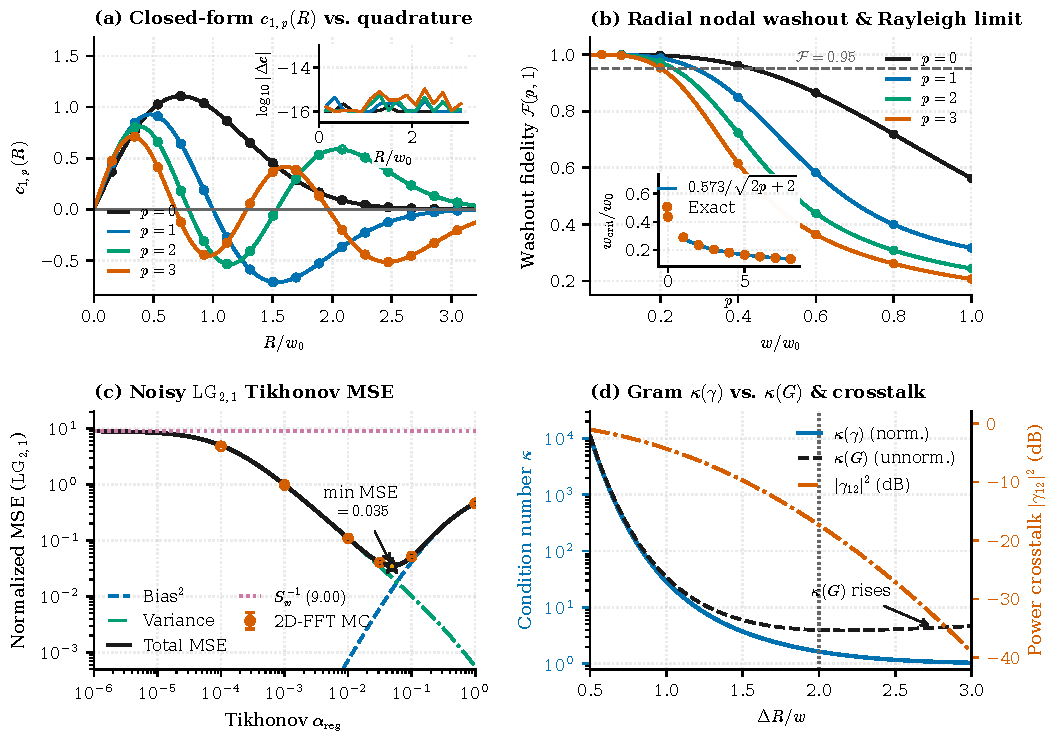
\includegraphics[width=0.76\textwidth]{fig2_laguerre_regularization.pdf}
\caption{Laguerre--Gaussian expansion, radial washout, regularized reconstruction, and Gram conditioning. (a) Analytical $c_{1,p}(R)$ (solid) vs.\ quadrature (circles) for $\mathrm{LG}_{p,1}$ ($p=0\text{--}3$, $w/w_0=0.25$); inset shows $\log_{10}\abs{\Delta c} < -14$. (b) Washout fidelity $\mathcal{F}(p,1,w/w_0)$ with Table~\ref{tab:fidelity} points (dots); inset compares exact $\mathcal{F}=0.95$ roots $w_{\mathrm{crit}}/w_0$ ($p=0\text{--}8$) against $0.573/\sqrt{2p+\abs{l}+1}$ ($l=1$). (c) Noisy $\mathrm{LG}_{2,1}$ MSE ($w/w_0=0.25, w k_{\max}=3.0, \mathrm{SNR}=20\,\mathrm{dB}$) decomposed into $\mathrm{Bias}^2$ and variance with 2D-FFT Monte Carlo (circles, $\pm 1\,\mathrm{SEM}$), achieving $\mathrm{MSE}_{\min} = 0.035$ ($0.0348$) at $\alpha_{\mathrm{reg}}^{\mathrm{opt}} = 0.0490$ vs.\ $9.00$ at $\alpha_{\mathrm{reg}}=0$. (d) Normalized $\kappa(\gamma)$ vs.\ unnormalized $\kappa(G)$ (left) and power crosstalk $\abs{\gamma_{12}}^2$ in dB (right) for Table~\ref{tab:gram_matrix}.}
\label{fig:laguerre_regularization}
\end{figure}

\subsection{Exact Closed-Form Expansion of \texorpdfstring{$\mathrm{LG}_{p,l}$}{LG\_\{p,l\}} Modes (\texorpdfstring{$p \ge 0$}{p >= 0})}
\label{subsec:analytic_lg_expansion}

Consider an arbitrary unit-$L^2$-normalized Laguerre--Gaussian mode $\mathrm{LG}_{p,l}$ with beam waist $w_0$ ($p \in \mathbb{Z}_{\ge 0}$, $l \in \mathbb{Z}$),
\begin{equation}
\psi_{p,l}(r,\phi) = N_{p,l}\!\left(\frac{\sqrt{2}r}{w_0}\right)^{\abs{l}} L_p^{\abs{l}}\!\left(\frac{2r^2}{w_0^2}\right) e^{-r^2/w_0^2 + il\phi},
\label{eq:lg_def}
\end{equation}
where $N_{p,l} = \sqrt{2p!/[\pi(p+\abs{l})!]}/w_0$, and frame projection coefficients $c_{l,p}(R) = \braket{\Phi_{l,R}}{\psi_{p,l}}$. Whereas Ref.~\cite{Ferreira2026} evaluated only $p=0$, the following theorem provides the exact finite algebraic solution for all $p \ge 0$.

\begin{theorem}[Exact closed-form expansion of $\mathrm{LG}_{p,l}$ modes]
\label{thm:c_lp_exact}
For all $p \in \mathbb{Z}_{\ge 0}$, $l \in \mathbb{Z}$, $w > 0$, and $w_0 > 0$, the continuous PVB projection $c_{l,p}(R) = \braket{\Phi_{l,R}}{\psi_{p,l}}$ is given by the $(p+1)$-term sum
\begin{equation}
c_{l,p}(R) = \mathcal{A}_{p,l}(R) \sum_{m=0}^p (-1)^m \binom{p+\abs{l}}{p-m} \eta^m L_m^{\abs{l}}(-z),
\label{eq:c_lp_exact}
\end{equation}
where $\eta = 2w^2/(w_0^2 + w^2)$, $z = R^2 w_0^2/[w^2(w_0^2 + w^2)]$, and
\begin{equation}
\mathcal{A}_{p,l}(R) = 2^{\frac{\abs{l}}{2}+1}\sqrt{\frac{p!}{(p+\abs{l})!}}\,\frac{R^{\abs{l}} w_0^{\abs{l}+1}}{(w_0^2 + w^2)^{\abs{l}+1}} e^{-\frac{R^2}{w_0^2 + w^2}}.
\label{eq:A_prefactor}
\end{equation}
These coefficients synthesize the frame-filtered $\mathrm{LG}_{p,l}$ mode exactly via
\begin{equation}
(S_w\psi_{p,l})(\mathbf{r}) = \int_0^\infty R\,dR\, c_{l,p}(R)\,\Phi_{l,R}(\mathbf{r}).
\label{eq:frame_synthesis_lg}
\end{equation}
\end{theorem}

The complete derivation—using the finite Laguerre polynomial expansion, Gradshteyn--Ryzhik formula 6.631.1 with $a_0 = 1/w^2 + 1/w_0^2$, $I_l = I_{\abs{l}}$, and Kummer's transformation—is given in Appendix~\ref{app:lg_expansion}. For $p=0$, Eq.~\eqref{eq:c_lp_exact} reduces to $c_{l,0}(R) = \mathcal{A}_{0,l}(R)$, which agrees with Ref.~\cite{Ferreira2026}'s $p=0$ overlap up to the unit-normalization factor $\norm{\Phi_{l,R}}_{L^2}^{-1}$ ($C_0$ vs.\ $N_{\abs{l}}$). Numerical quadrature confirms Eqs.~\eqref{eq:c_lp_exact}--\eqref{eq:frame_synthesis_lg} to $<3 \times 10^{-15}$ [Fig.~\ref{fig:laguerre_regularization}(a)]. Exact inversion of Eq.~\eqref{eq:frame_synthesis_lg} holds only at $\alpha_{\mathrm{reg}}=0$ on $\mathcal{H}_{k_{\max}}$ (via projected duals), whereas $S_{w,\alpha_{\mathrm{reg}}}^{-1}$ ($\alpha_{\mathrm{reg}} > 0$) trades bias for noise stability per Proposition~\ref{prop:tikhonov_dual}.

\subsection{Radial Resolution Limits and Nodal Washout}
\label{subsec:nodal_washout}

Because $\psi_{p,l}$ possesses $p$ concentric radial nodes~\cite{Allen1992,Siegman1986,Walborn2010}, Gaussian smoothing by $S_w$ washes out fine radial oscillations when $w$ becomes comparable to the nodal spacing. Using the Fourier-domain form of Eq.~\eqref{eq:fourier_diag} with $u = w_0^2 k_\perp^2/2$, $a = w^2/w_0^2$, and normalized spectral density $\rho_{p,l}(u) = [p!/(p+\abs{l})!]u^{\abs{l}} e^{-u}[L_p^{\abs{l}}(u)]^2$, the reconstruction fidelity $\mathcal{F}(p,l,w/w_0) = \abs{\braket{\psi_{p,l}}{S_w\psi_{p,l}}}^2/\norm{S_w\psi_{p,l}}_{L^2}^2$ evaluates to
\begin{equation}
\mathcal{F}(p,l,w/w_0) = \frac{\left(\int_0^\infty e^{-au}\,\rho_{p,l}(u)\,du\right)^2}{\int_0^\infty e^{-2au}\,\rho_{p,l}(u)\,du}.
\label{eq:fidelity_fourier}
\end{equation}
Table~\ref{tab:fidelity} lists exact values from Eq.~\eqref{eq:fidelity_fourier} for $l=1$, matching exact rational fractions at $w/w_0 = 1.00$ ($9/16$, $81/256$, $18225/74752$, and $8037225/38862848$).

\begin{table}[htbp]
\caption{Exact reconstruction fidelity $\mathcal{F}(p, l=1, w/w_0)$ of $\mathrm{LG}_{p,1}$ modes under the PVB frame operator $S_w$ across relative ring widths $w/w_0$. At $w/w_0 = 1.00$, values match the exact rationals $9/16$, $81/256$, $18225/74752$, and $8037225/38862848$.}
\label{tab:fidelity}
\begin{ruledtabular}
\setlength{\tabcolsep}{3pt}
\begin{tabular}{ccccc}
$w / w_0$ & $\mathcal{F}(p=0)$ & $\mathcal{F}(p=1)$ & $\mathcal{F}(p=2)$ & $\mathcal{F}(p=3)$ \\
\hline
0.05 & 0.99999 & 0.99995 & 0.99989 & 0.99980 \\
0.10 & 0.99980 & 0.99921 & 0.99822 & 0.99683 \\
0.20 & 0.99704 & 0.98782 & 0.97282 & 0.95276 \\
0.40 & 0.96231 & 0.84935 & 0.72301 & 0.61610 \\
0.60 & 0.86477 & 0.58216 & 0.43953 & 0.36419 \\
0.80 & 0.71861 & 0.39960 & 0.30831 & 0.26129 \\
1.00 & 0.56250 & 0.31641 & 0.24381 & 0.20681 \\
\end{tabular}
\end{ruledtabular}
\end{table}

\begin{corollary}[Generalized radial Rayleigh criterion]
\label{cor:rayleigh_radial}
Retaining reconstruction fidelity $\mathcal{F}(p,l,w/w_0) \ge 0.95$ requires: (i) for $p = 0$, the exact closed-form bound
\begin{equation}
w \le w_{\mathrm{crit}}(0,l) = \left[\left(1 - 0.95^{1/(\abs{l}+1)}\right)^{-1/2} - 1\right]^{-1/2} w_0,
\label{eq:rayleigh_p0}
\end{equation}
yielding $0.5367\,w_0$ ($l=0$), $0.4350\,w_0$ ($l=1$), and $0.3869\,w_0$ ($l=2$); and (ii) for $p \ge 1$, the nodal Rayleigh threshold
\begin{equation}
w \lesssim w_{\mathrm{crit}}(p,l) \approx \frac{0.573}{\sqrt{2p + \abs{l} + 1}}\,w_0 \qquad (p \ge 1),
\label{eq:rayleigh_radial}
\end{equation}
approaching the large-$p$ arcsine-law asymptote $I_0(c)^2/I_0(2c) = 0.95 \implies \sqrt{c} = 0.5724$ (above the 2nd-cumulant Taylor coefficient $0.10^{1/4} = 0.5623$).
\end{corollary}
\begin{proof}
At $p=0$, Eq.~\eqref{eq:fidelity_fourier} integrates to $\mathcal{F}(0,l,w/w_0) = [(1+2a)/(1+a)^2]^{\abs{l}+1}$; solving $\mathcal{F} = 0.95$ for $a = w^2/w_0^2$ yields Eq.~\eqref{eq:rayleigh_p0}. For $p \ge 1$, $\operatorname{Var}_{\rho_{p,l}}(u) = 2p^2 + 2p\abs{l} + 2p + \abs{l} + 1 \approx \frac{1}{2}(2p+\abs{l}+1)^2$ sets the $(2p+\abs{l}+1)^{-1/2}$ scaling in Eq.~\eqref{eq:rayleigh_radial}, while direct root-finding at $l=1$ gives $w_{\mathrm{crit}}\sqrt{2p+\abs{l}+1}/w_0 = 0.5806\,(p=1), 0.5759\,(p=2), 0.5744\,(p=3), 0.5727\,(p=10)$, converging to $0.5724$ [Fig.~\ref{fig:laguerre_regularization}(b) inset].
\end{proof}

\subsection{Optimal Radial Discretization and Normalized Gram Spectrum}
\label{subsec:gram_sampling}

Sampling $N$ concentric ring radii $R_n = R_{\min} + (n-1)\Delta R$ ($n=1,\dots,N$) at fixed $l$ defines the unnormalized Gram matrix $G_{nm} = \braket{\Phi_{l,R_n}}{\Phi_{l,R_m}}$ from Eq.~\eqref{eq:overlap_closed} and the unit-normalized channel Gram matrix
\begin{equation}
\gamma_{nm} = \frac{G_{nm}}{\sqrt{G_{nn} G_{mm}}} = \braket{\psi_{l,R_n}}{\psi_{l,R_m}}.
\label{eq:gram_normalized}
\end{equation}
Because $G_{nn} \approx (2\pi R_n^2 w^2)^{-1/2}$ decays with $R_n$, $\kappa(G) = \lambda_{\max}(G)/\lambda_{\min}(G)$ grows artificially with $N$ even when rings decouple (e.g., at $N=120, \Delta R = 2.0w$, $\kappa(G) = 80.02$ whereas $\kappa(\gamma) = 1.741$). True channel conditioning is governed solely by $\gamma_{nm}$ in Eq.~\eqref{eq:gram_normalized}. In the large-ring annular regime $R_{\min} \gg w, \abs{l}w/2$, Hankel asymptotics yield the adjacent field overlap
\begin{equation}
\gamma_{n,n+1} \approx \exp\!\left(-\frac{\Delta R^2}{2w^2}\right),
\label{eq:crosstalk_asymptotic}
\end{equation}
and power crosstalk $\abs{\gamma_{n,n+1}}^2 \approx \exp(-\Delta R^2/w^2)$. Near the core, Eq.~\eqref{eq:crosstalk_asymptotic} breaks down (e.g., at $R_{\min} = 0.2w, l=1, \Delta R = 2.0w$, exact $\gamma_{12} = 34.76\%$ vs.\ $e^{-2} = 13.53\%$).

\begin{proposition}[Discrete radial sampling and normalized Gram bound]
\label{prop:channel_capacity}
In the annular regime $R_{\min} \gg w, \abs{l}w/2$, enforcing $\Delta R \ge 2.0\,w$ maintains normalized Gram conditioning $\kappa(\gamma) \le 1.65$ ($N=6$; $\le 1.75$ for $N=120$), adjacent field overlap $\le 13.6\%$ (power crosstalk $\le 1.84\%$, $\ge 17.36\,\mathrm{dB}$ isolation), and normalized zero-forcing penalties $\le 0.42\,\mathrm{dB}$ for $N=6$ ($0.14\,\mathrm{dB}$ correlated, $0.412\,\mathrm{dB}$ AWGN) and $< 0.50\,\mathrm{dB}$ for all $N$ ($0.491\,\mathrm{dB}$ at $N=120$; $0.495\,\mathrm{dB}$ Toeplitz limit). Across radial aperture $\mathcal{W} = R_{\max} - R_{\min}$, the maximum stable channel count is
\begin{equation}
N_{\max} \approx \left\lfloor \frac{\mathcal{W}}{2w} \right\rfloor + 1.
\label{eq:channel_capacity}
\end{equation}
\end{proposition}

Table~\ref{tab:gram_matrix}, Eq.~\eqref{eq:channel_capacity}, and Fig.~\ref{fig:laguerre_regularization}(d) confirm monotonic convergence of $\kappa(\gamma)$ ($\kappa > 10^4$ only at $\Delta R \le 0.5\,w$), reaching quasi-orthogonal isolation ($27.13\,\mathrm{dB}$ power isolation, $4.40\%$ amplitude overlap, $\kappa(\gamma) = 1.172$) at $\Delta R = 2.5\,w$.

\begin{table}[htbp]
\caption{Normalized Gram conditioning, adjacent field/power crosstalk, and zero-forcing (ZF) noise-enhancement penalties for $N = 6$ discrete radial PVB channels ($w = 0.5\,\ell_0$, $l = 1$, $R_{\min} = 2.0\,\ell_0$, in arbitrary reference length units $\ell_0$). Unnormalized $\kappa(G)$ is shown alongside $\kappa(\gamma)$ to illustrate spurious norm-induced growth.}
\label{tab:gram_matrix}
\begin{ruledtabular}
\footnotesize
\setlength{\tabcolsep}{1pt}
\begin{tabular}{ccccccccc}
$\Delta R / w$ & $\Delta R\,(\ell_0)$ & $\abs{\gamma_{12}}$ & $\abs{\gamma_{12}}^2$ (Iso.) & $\kappa(\gamma)$ & $\kappa(G)$ & $\operatorname{Tr}(\gamma^{-1})/N$ & $\operatorname{Tr}(\gamma^{-2})/N$ & Regime \\
\hline
0.50 & 0.250 & $88.26\%$ & $77.91\%$ ($1.08$~dB) & $1.086\times 10^4$ & $1.123\times 10^4$ & $502.0$ ($27.01$~dB) & $1.364\times 10^6$ ($61.35$~dB) & Ill-conditioned \\
1.00 & 0.500 & $60.68\%$ & $36.83\%$ ($4.34$~dB) & $28.80$ & $34.30$ & $3.418$ ($5.34$~dB) & $30.14$ ($14.79$~dB) & Ill-conditioned \\
1.50 & 0.750 & $32.50\%$ & $10.56\%$ ($9.76$~dB) & $3.723$ & $5.960$ & $1.237$ ($0.92$~dB) & $1.890$ ($2.76$~dB) & Transition \\
2.00 & 1.000 & $13.55\%$ & $1.84\%$ ($17.36$~dB) & $1.645$ & $3.959$ & $1.032$ ($0.14$~dB) & $1.099$ ($0.41$~dB) & Optimal \\
2.50 & 1.250 & $4.40\%$ & $0.194\%$ ($27.13$~dB) & $1.172$ & $4.096$ & $1.003$ ($0.01$~dB) & $1.010$ ($0.04$~dB) & Quasi-orthogonal \\
3.00 & 1.500 & $1.11\%$ & $0.012\%$ ($39.07$~dB) & $1.041$ & $4.646$ & $1.000$ ($0.00$~dB) & $1.001$ ($0.00$~dB) & Quasi-orthogonal \\
\end{tabular}
\end{ruledtabular}
\end{table}

\section{Quantitative Utility in Classical and Quantum Optics}
\label{sec:optics_utility}

\subsection{Classical Optics: Noisy Reconstruction, RCF Links, and Turbulence}
\label{subsec:classical_utility}

\paragraph*{Worked noisy $\mathrm{LG}_{2,1}$ Tikhonov reconstruction.}
To make Proposition~\ref{prop:tikhonov_dual} and Theorem~\ref{thm:c_lp_exact} concrete, consider reconstructing $\mathrm{LG}_{2,1}$ ($w/w_0 = 0.25$, $w k_{\max} = 3.0$) from $\psi_{\mathrm{meas}} = S_w\psi_{2,1} + \eta$, where $\eta$ is bandlimited white noise of power $P_\eta = 0.01$ (input $\mathrm{SNR} = 20\,\mathrm{dB}$). By Parseval's theorem, the normalized reconstruction error $\mathrm{MSE}(\alpha_{\mathrm{reg}}) = \mathrm{Bias}^2(\alpha_{\mathrm{reg}}) + \mathrm{Var}(\alpha_{\mathrm{reg}})$ splits analytically into
\begin{align}
\mathrm{Bias}^2 &= \int_0^\infty \left[\frac{\alpha_{\mathrm{reg}}}{\widetilde{G}_w^2(u) + \alpha_{\mathrm{reg}}}\right]^2 \rho_{2,1}(u)\,du, \nonumber \\
\mathrm{Var} &= \frac{P_\eta}{(w k_{\max})^2}\left[\frac{1}{e^{-w^2 k_{\max}^2}+\alpha_{\mathrm{reg}}} - \frac{1}{1+\alpha_{\mathrm{reg}}}\right],
\label{eq:tikhonov_mse_worked}
\end{align}
with $\widetilde{G}_w^2(u) = e^{-2a u}$. Evaluating Eq.~\eqref{eq:tikhonov_mse_worked}, unregularized inversion ($\alpha_{\mathrm{reg}} = 0$) suffers $\mathrm{MSE}_0 = 9.002$, whereas Tikhonov regularization attains a unique interior minimum $\mathrm{MSE}_{\min} = 0.03481$ ($\mathrm{Bias}^2 = 0.01326$, $\mathrm{Var} = 0.02155$) at $\alpha_{\mathrm{reg}}^{\mathrm{opt}} = 0.04902$—a $258.6\times$ ($24.1\,\mathrm{dB}$) MSE suppression, confirmed by $256\times 256$ 2D-FFT Monte Carlo simulations [Fig.~\ref{fig:laguerre_regularization}(c)].

\paragraph*{Sturm--Liouville RCF coupling and SDM equalization penalties.}
Solving the 1D scalar Helmholtz Sturm--Liouville eigenvalue problem for a step-index RCF ($r_1 = 6.0\,\mu\mathrm{m}, r_2 = 9.0\,\mu\mathrm{m}, n_{\mathrm{clad}} = 1.444, \Delta n = 0.033, \lambda = 1550\,\mathrm{nm}$), the physical PVB ($w = 1.72\,\mu\mathrm{m}$) achieves fiber-mode overlap $\eta_{\mathrm{PVB}} \ge 95.87\%$ across $l=0\text{--}8$ (mean $98.52\%$, rising to $99.40\%$ at $w_{\mathrm{opt}} = 1.92\,\mu\mathrm{m}$) [Fig.~\ref{fig:optics_utility}(a)]. At $l=4$, PVB coupling yields a $+6.90\,\mathrm{dB}$ analytical gain over $\mathrm{LG}_{0,4}$ ($w_0 = 3.22\,\mu\mathrm{m}$, $\eta_{\mathrm{LG}} = 0.2026$), closely matching Villalba \emph{et al.}'s $6.83\,\mathrm{dB}$ experiment~\cite{Villalba2023}.

When demultiplexing $N=6$ discrete radial channels via zero-forcing or minimum mean-square error (MMSE) equalization~\cite{Willner2015,Wang2019} on $\gamma_{nm}$ (Proposition~\ref{prop:channel_capacity}), the normalized per-channel noise-enhancement factors under correlated frame-projection noise ($\mathbb{E}[\eta\eta^\dagger] = \sigma^2 \gamma$) and post-projection additive white Gaussian noise (AWGN, $\mathbb{E}[\eta\eta^\dagger] = \sigma^2 I$) are, respectively,
\begin{equation}
\mathcal{P}_{\mathrm{corr}} = \frac{1}{N}\operatorname{Tr}(\gamma^{-1}), \qquad \mathcal{P}_{\mathrm{AWGN}} = \frac{1}{N}\operatorname{Tr}(\gamma^{-2}).
\label{eq:zf_penalties}
\end{equation}
Evaluating Eq.~\eqref{eq:zf_penalties} at $\Delta R = 2.0\,w$ yields $\mathcal{P}_{\mathrm{corr}} = 1.032$ ($0.14\,\mathrm{dB}$) and $\mathcal{P}_{\mathrm{AWGN}} = 1.099$ ($0.41\,\mathrm{dB}$), falling to $1.003$ ($0.01\,\mathrm{dB}$) and $1.010$ ($0.04\,\mathrm{dB}$) at $\Delta R = 2.5\,w$ (Table~\ref{tab:gram_matrix}), leaving the $l=4$ OOK bit-error rate (BER) virtually unaffected [Fig.~\ref{fig:optics_utility}(a) inset].

\begin{figure}[htbp]
\centering
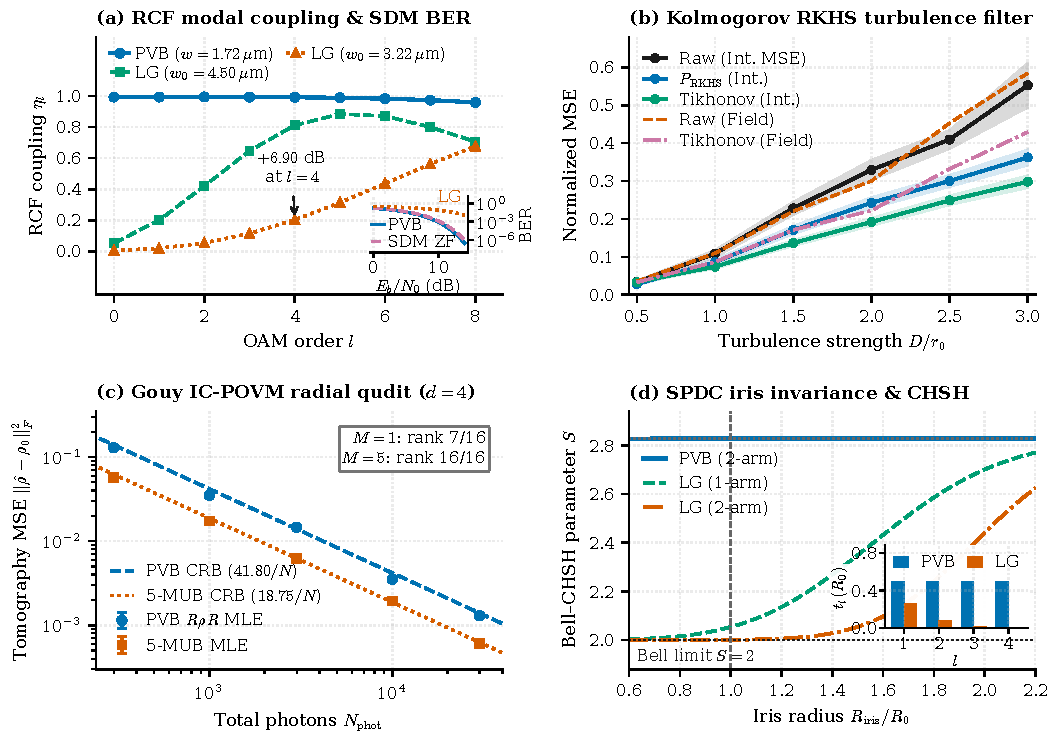
\includegraphics[width=0.76\textwidth]{fig3_optics_utility.pdf}
\caption{Classical and quantum optics utility of PVB completeness. (a) Sturm--Liouville RCF coupling $\eta_l$ ($r_1=6.0\,\mu\mathrm{m}, r_2=9.0\,\mu\mathrm{m}, \Delta n=0.033, \lambda=1550\,\mathrm{nm}$) for PVBs ($w=1.72\,\mu\mathrm{m}$, mean $0.985$) vs.\ $\mathrm{LG}_{0,l}$ ($w_0=4.50, 3.22\,\mu\mathrm{m}$), achieving $+6.90\,\mathrm{dB}$ gain at $l=4$; inset shows $l=4$ OOK BER with the $0.41\,\mathrm{dB}$ AWGN ZF penalty at $\Delta R = 2.0w$. (b) Intensity MSE (solid, $\pm 1\,\mathrm{SEM}$) and field MSE (dashed/dash-dotted) over 40 Kolmogorov phase screens ($D=3.0\,\mathrm{mm}, z=0.5\,\mathrm{m}$) for raw, $P_{\mathrm{RKHS}}$, and Tikhonov ($\alpha_{\mathrm{reg}}=0.0183$) filtering. (c) Passive $M=5$ Gouy IC-POVM radial qudit tomography ($d=4, l=1, w/w_0=0.25$, rank $16/16$ vs.\ $7/16$ at $M=1$): $R\rho R$ MLE MSE (circles, 30 trials) tracks CRB $41.80/N_{\mathrm{phot}}$ alongside 5-MUB tomography ($18.75/N_{\mathrm{phot}}$). (d) SPDC Bell--CHSH $S$ vs.\ circular-iris radius $R_{\mathrm{iris}}/R_0$ for $(l=1,4)$ ($w=0.1 R_0$, LG $w_0=\sqrt{2}R_0$); inset shows $t_{1..4}(R_0)$ ($0.4999\text{--}0.4984$ PVB vs.\ $0.2642\text{--}0.0037$ LG).}
\label{fig:optics_utility}
\end{figure}

\paragraph*{RKHS filtering under Kolmogorov atmospheric turbulence.}
Atmospheric turbulence scatters transverse spatial modes into high-$k_\perp$ speckles~\cite{Paterson2005,TylerBoyd2009,AndrewsPhillips2005}. Evaluating $40$ subharmonic-corrected $256\times 256$ Kolmogorov phase screens~\cite{Lane1992} ($D_{\mathrm{ap}} = 3.0\,\mathrm{mm}, z = 0.5\,\mathrm{m}, R_0 = 1.0\,\mathrm{mm}, w = 0.25\,\mathrm{mm}, k_{\max} = 8.0\,\mathrm{rad/mm}, \alpha_{\mathrm{reg}} = e^{-(wk_{\max})^2} = 0.0183$), both the RKHS projector $P_{\mathrm{RKHS}} = P_{k_{\max}}$~\cite{PaulsenRaghupathi2016} and Tikhonov filtering $S_{w,\alpha_{\mathrm{reg}}}^{-1}S_w$ consistently suppress turbulence distortion across $D/r_0 \in [0.5,3.0]$ [Fig.~\ref{fig:optics_utility}(b)]. At $D/r_0 = 3.0$, raw field MSE drops from $0.585$ to $0.471$ ($P_{\mathrm{RKHS}}$) and $0.429$ (Tikhonov), while intensity MSE drops from $0.553$ to $0.362$ and $0.298$.

\subsection{Quantum Optics: Multi-Plane IC-POVM Tomography and Iris Invariance}
\label{subsec:quantum_utility}

\paragraph*{Passive multi-plane Gouy-diverse IC-POVM radial qudit tomography.}
On a $d$-dimensional radial qudit subspace $\mathcal{H}_d^{(l)} = \operatorname{span}\{\ket{\psi_{p,l}}\}_{p=0}^{d-1}$ at fixed $l$, single-plane ($z=0$) PVB projections are \emph{not} informationally complete (IC): because $c_{l,p}(R) \in \mathbb{R}$, the measurement operators span only $2d-1 < d^2$ degrees of freedom (rank $7/16$ at $d=4$). Dividing the beam passively across $M \ge d+1$ propagation planes with distinct Gouy phases $\zeta_m = \arctan(z_m/z_R)$ breaks this real-polynomial degeneracy via the POVM elements~\cite{Renes2004}
\begin{align}
\Pi_{m,k} &= \frac{R_k \Delta R}{M}\ket{\phi_{m,k}}\bra{\phi_{m,k}}, \nonumber \\
\braket{\psi_{p,l}}{\phi_{m,k}} &= e^{-i(2p+\abs{l}+1)\zeta_m} c_{l,p}(R_k),
\label{eq:ic_povm_elements}
\end{align}
completed by the residual outcome $\Pi_{\mathrm{res}} = I_d - \sum_{m,k}\Pi_{m,k}$ ($\lambda_{\max}(\sum \Pi_{m,k}) = 0.9050 < 1$). For $d=4, l=1, w/w_0=0.25, M=5$ ($\zeta_m \in [0,0.45\pi]$) and 40 midpoint bins $R_k \in (0, 3.5\,w_0]$, Eq.~\eqref{eq:ic_povm_elements} achieves full operator rank $16/16$ with minimum Fisher eigenvalue $\lambda_{\min}(\mathbf{F}) = 0.1261$ and single-photon Cram\'er--Rao bound (CRB) at $\rho_0 = I_4/4$:
\begin{equation}
\operatorname{Tr}\!\left[\mathbf{F}^{-1}\right] = 41.80 \quad (\text{with }\Pi_{\mathrm{res}};\; 42.96\text{ without}),
\label{eq:fisher_crb}
\end{equation}
versus $18.75$ for 5 sequential mutually unbiased bases (MUBs), enabling passive single-shot tomography without active SLM switching. Thirty-trial iterative $R\rho R$ maximum-likelihood estimation (MLE)~\cite{Lvovsky2004} tracks Eq.~\eqref{eq:fisher_crb} cleanly as $41.80/N_{\mathrm{phot}}$ [Fig.~\ref{fig:optics_utility}(c)].

\paragraph*{$l$-invariant QKD footprint and SPDC circular-iris Bell--CHSH preservation.}
In high-dimensional QKD and spontaneous parametric down-conversion (SPDC)~\cite{Cerf2002,LawEberly2004,Walborn2010,Mirhosseini2015}, finite circular apertures clip high-$\abs{l}$ LG modes via $t_l^{\mathrm{LG}}(R_{\mathrm{iris}}) = P(\abs{l}+1, 2R_{\mathrm{iris}}^2/w_0^2)$, whereas physical PVBs preserve $l$-independent throughput. For $R_0 = 1, w = 0.1, R_{\mathrm{iris}} = R_0$ (vs.\ peak-matched $\mathrm{LG}_{0,l}$ with $w_0 = \sqrt{2}R_0$), exact quadrature gives $t_{1..4}^{\mathrm{PVB}} = [0.4999, 0.4996, 0.4991, 0.4984]$, eliminating $l$-dependent QKD side-channels, whereas $t_{1..4}^{\mathrm{LG}} = [0.2642, 0.0803, 0.0190, 0.0037]$ [Fig.~\ref{fig:optics_utility}(d) inset]. For the two-photon Bell state $\ket{\Psi} = (\ket{1,-1} + \ket{4,-4})/\sqrt{2}$ passing through circular irises of radius $R_{\mathrm{iris}}$, the post-selected Bell--CHSH parameter~\cite{Clauser1969} reads
\begin{equation}
S(R_{\mathrm{iris}}) = 2\sqrt{1 + \mathcal{V}^2(R_{\mathrm{iris}})}, \qquad \mathcal{V} = \frac{2\sqrt{t_1 t_4}}{t_1 + t_4},
\label{eq:iris_chsh}
\end{equation}
for single-arm truncation (replacing $t_l \to t_l^2$ for symmetric two-arm irises). By Eq.~\eqref{eq:iris_chsh} at $R_{\mathrm{iris}} = R_0$, PVBs maintain near-maximal violation $S_{\mathrm{PVB}} = 2.8284$ (two-arm), whereas LG modes collapse to $S_{\mathrm{LG}} = 2.0532$ (one-arm) and $2.0008$ (two-arm) [Fig.~\ref{fig:optics_utility}(d)].

\section{Conclusions}
\label{sec:conclusions}

Addressing the four questions in Sec.~\ref{sec:intro}, we established the operator-theoretic framework of physical PVBs as continuous Hilbert frames. While azimuthal OAM sectors remain strictly orthogonal ($\mathcal{H} = \bigoplus_{l\in\mathbb{Z}}\mathcal{H}_l$), finite width $w > 0$ induces an isotropic Gaussian convolution frame operator $S_w$ with vanishing lower bound on $L^2(\mathbb{R}^2)$ and sharp Paley--Wiener bounds $A = \exp(-w^2 k_{\max}^2/2), B = 1$ on $\mathcal{H}_{k_{\max}}$ (Remark~\ref{rem:propagation} and Theorem~\ref{thm:pw_bounds}). We constructed the projected Tikhonov dual frame, derived the exact $(p+1)$-term closed-form expansion $c_{l,p}(R)$ for all $\mathrm{LG}_{p,l}$ modes ($p \ge 0$), established the revised Rayleigh threshold $w_{\mathrm{crit}} \approx 0.573\,w_0/\sqrt{2p+\abs{l}+1}$ ($p \ge 1$, Corollary~\ref{cor:rayleigh_radial}) and exact $p=0$ formula, and proved normalized Gram stability ($\kappa(\gamma) = 1.645$, $17.36\,\mathrm{dB}$ isolation at $\Delta R = 2.0\,w$, Proposition~\ref{prop:channel_capacity}). Our classical and quantum benchmarks validate PVB frames across noisy reconstruction, RCF/SDM links, turbulence filtering, passive IC-POVM tomography, and iris-invariant entanglement. All analytical identities and benchmarks in Secs.~\ref{sec:frame_formalism}--\ref{sec:optics_utility} were independently verified via reproducible Python symbolic and numerical routines.

\begin{acknowledgments}
This research was conducted as a collaborative effort between the sole human author, Sebasti\'an Ayala, and the generative artificial intelligence system Gemini (in its Antigravity IDE mode). Sebasti\'an Ayala conceived the research program, formulated the physical hypotheses and optical boundary conditions, directed all analytical and numerical investigations, and independently verified every derivation, simulation result, and bibliographic record, assuming full responsibility for the scientific content of this work in compliance with American Physical Society (APS) editorial policies. Gemini (in its Antigravity IDE mode) provided substantive assistance with symbolic calculus, asymptotic analysis, reproducible numerical verification scripting, vector figure generation, and manuscript drafting.
\end{acknowledgments}

\appendix
\section{Derivation of the Closed-Form Expansion Coefficients \texorpdfstring{$c_{l,p}(R)$}{c\_\{l,p\}(R)}}
\label{app:lg_expansion}

Evaluating $c_{l,p}(R) = \braket{\Phi_{l,R}}{\psi_{p,l}}$ from Eqs.~\eqref{eq:pvb_mode} and~\eqref{eq:lg_def} and integrating over $\phi \in [0,2\pi)$ gives
\begin{align}
c_{l,p}(R) &= 2\pi C_0 N_{p,l} e^{-R^2/w^2} \int_0^\infty r\,dr\, e^{-a_0 r^2} I_{\abs{l}}(\beta r) \nonumber \\
&\quad \times \left(\frac{\sqrt{2}r}{w_0}\right)^{\abs{l}} L_p^{\abs{l}}\!\left(\frac{2r^2}{w_0^2}\right),
\label{eq:app_c_int}
\end{align}
where $a_0 = 1/w^2 + 1/w_0^2$, $\beta = 2R/w^2$, $N_{p,l} = \sqrt{2p!/[\pi(p+\abs{l})!]}/w_0$, and we invoked $I_l(\beta r) = I_{\abs{l}}(\beta r)$ for $l \in \mathbb{Z}$. Substituting the finite polynomial $L_p^{\abs{l}}(2r^2/w_0^2) = \sum_{m=0}^p (-1)^m \binom{p+\abs{l}}{p-m} (m!)^{-1} (2/w_0^2)^m r^{2m}$ separates Eq.~\eqref{eq:app_c_int} into a $(p+1)$-term sum of radial integrals:
\begin{align}
\mathcal{J} &= \left(\frac{\sqrt{2}}{w_0}\right)^{\abs{l}} \sum_{m=0}^p \frac{(-1)^m}{m!}\binom{p+\abs{l}}{p-m}\left(\frac{2}{w_0^2}\right)^m \nonumber \\
&\quad \times \int_0^\infty r^{\abs{l}+2m+1} e^{-a_0 r^2} I_{\abs{l}}(\beta r)\,dr.
\label{eq:app_J_sum}
\end{align}
Each radial integral is evaluated via formula 6.631.1 of Gradshteyn and Ryzhik~\cite{Gradshteyn2014}, analytically continued via $J_\nu(i\beta x) = i^\nu I_\nu(\beta x)$ for $\operatorname{Re}(a_0) > 0$ and $\operatorname{Re}(\mu+\nu) > 0$:
\begin{align*}
\int_0^\infty x^{\mu-1} e^{-a_0 x^2} I_\nu(\beta x)\,dx &= \frac{\beta^\nu \Gamma\left(\frac{\mu+\nu}{2}\right)}{2^{\nu+1} a_0^{(\mu+\nu)/2} \Gamma(\nu+1)} \\
&\quad \times {_1F_1}\!\left(\frac{\mu+\nu}{2}; \nu+1; \frac{\beta^2}{4a_0}\right).
\end{align*}
Setting $\nu = \abs{l} \ge 0$ and $\mu = \abs{l} + 2m + 2$ gives $(\mu+\nu)/2 = \abs{l} + m + 1$, yielding
\begin{align}
&\int_0^\infty r^{\abs{l}+2m+1} e^{-a_0 r^2} I_{\abs{l}}(\beta r)\,dr \nonumber \\
&\quad = \frac{\beta^{\abs{l}}(\abs{l}+m)!}{2^{\abs{l}+1} a_0^{\abs{l}+m+1}\abs{l}!}\,{_1F_1}\!\left(\abs{l}+m+1; \abs{l}+1; \frac{\beta^2}{4a_0}\right).
\label{eq:app_hypergeom}
\end{align}
Applying Kummer's first transformation ${_1F_1}(a;b;z) = e^z {_1F_1}(b-a;b;-z)$ to Eq.~\eqref{eq:app_hypergeom} sets $b - a = -m$, terminating the series as
\begin{equation}
{_1F_1}(-m; \abs{l}+1; -z) = \frac{m!\,\abs{l}!}{(\abs{l}+m)!} L_m^{\abs{l}}(-z),
\label{eq:app_kummer_laguerre}
\end{equation}
with $z = \beta^2/(4a_0) = R^2 w_0^2/[w^2(w_0^2+w^2)]$. Combining $-R^2/w^2 + \beta^2/(4a_0) = -R^2/(w_0^2 + w^2)$, identifying $[2/(a_0 w_0^2)]^m = \eta^m$, and matching $2\pi C_0 N_{p,l}\beta^{\abs{l}} 2^{-(\abs{l}+1)} a_0^{-(\abs{l}+1)} (\sqrt{2}/w_0)^{\abs{l}} e^{-R^2/(w_0^2+w^2)} = \mathcal{A}_{p,l}(R)$, the factorials $m!$ and $(\abs{l}+m)!$ cancel between Eqs.~\eqref{eq:app_J_sum}--\eqref{eq:app_kummer_laguerre}, proving Eqs.~\eqref{eq:c_lp_exact}--\eqref{eq:A_prefactor} of Theorem~\ref{thm:c_lp_exact}.

\bibliography{references}

\end{document}
